
The results of performance metrics  
measurements (\ref{sec:performance-metrics}) of Zigbee and Thread
networks are presented and discussed throughout this chapter. Tests
were executed on networks consisting of 7 devices
and followed the procedures described in chapter \ref{chap:research_methodology}.

\section{Latency}
\label{sec:latency}

\subsection{Latency in Thread networks}

All Thread latency measurement results are gathered in the table \ref{table:thread_latency}.

\subsubsection*{Relation between latency and the number of hops}

Let's first have a look at the plots of latency in Thread network 
(Fig. \ref{fig:thread_latency_all}).

\begin{figure}[H]
    \centering
    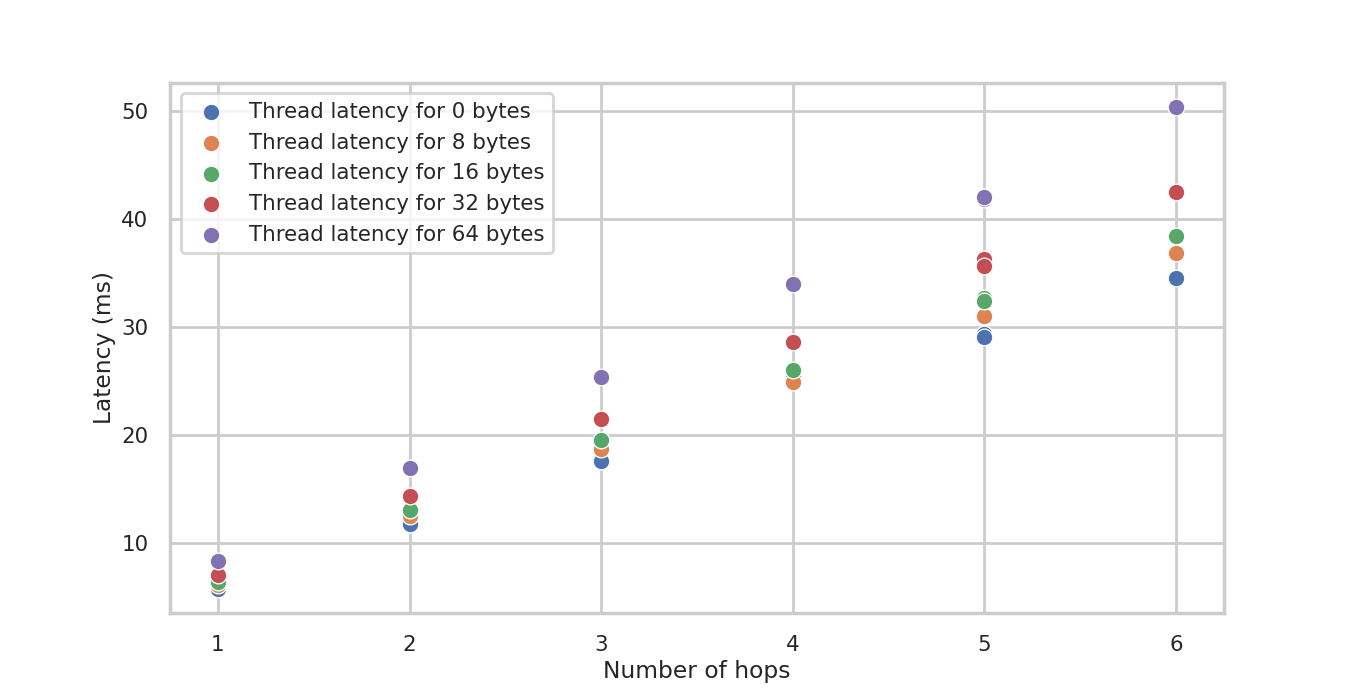
\includegraphics[scale=0.45]{images/Thread_Latency_all.png}
    \caption{Latency in Thread network dependent on the number of hops.}
    \label{fig:thread_latency_all}
\end{figure}

The number of hops, a packet must be passed through is the most
significant factor affecting the latency. It is clearly noticeable,
that additional hop adds roughly the same amount of time
to the overall packet delivery delay. It means that the latency is affected the most  
by the routing inside the network. To sum up, \textbf{the relation
between latency and the number of hops can be expressed as a
product of single hop delay and the number of hops.}

\subsubsection*{Relation between latency and payload length}
The length of a packet contributes to the packet delivery delay 
as well as the number of hops. The former relation is shown
in \ref{fig:thread_latency_length}.

\begin{figure}[H]
    \centering
    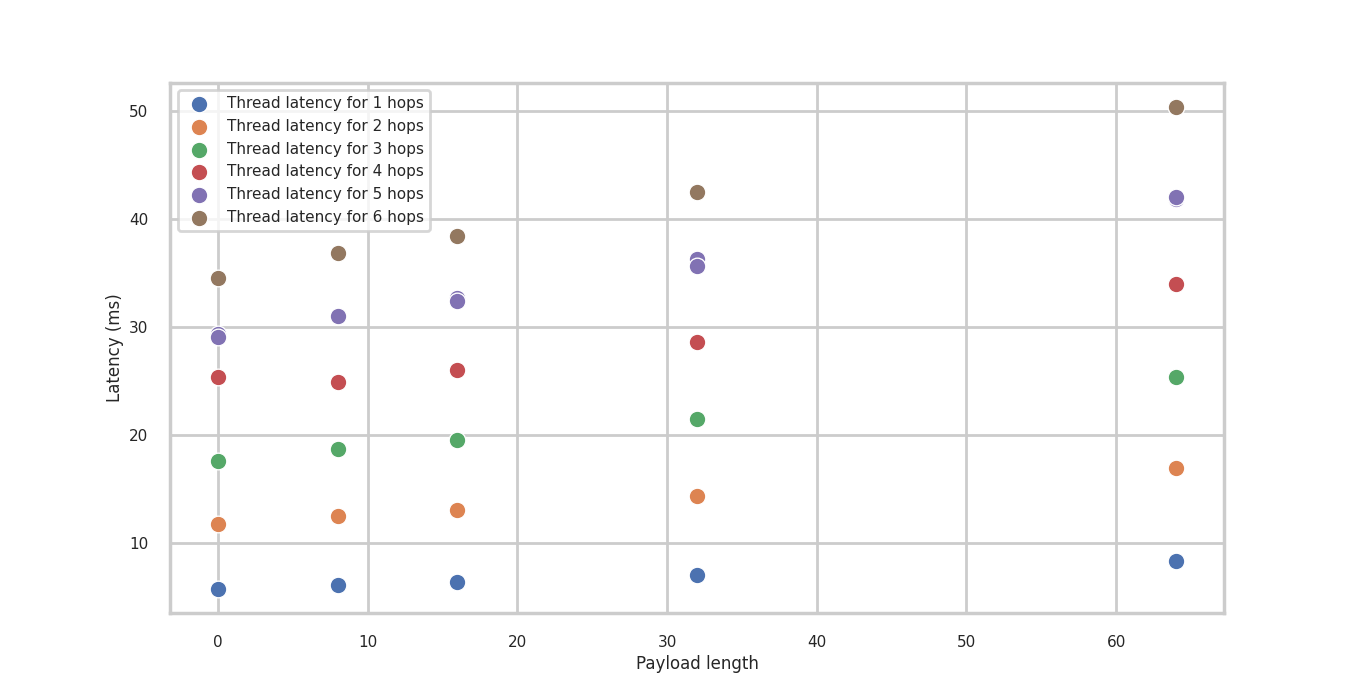
\includegraphics[scale=0.45]{images/Thread_Latency_vs_length.png}
    \caption{Latency in Thread network dependent on the payload length. }
    \label{fig:thread_latency_length}
\end{figure}

In this case, 
increasing the payload length does not affect the latency as much
as routing. However, the delay of 64 bytes long payload is a 
latency of 0 bytes long payload doubled. Looking at the plot and
the table of results (\ref{table:thread_latency}), \textbf{the 
single hop latency can be estimated between 5 and 9 
milliseconds}.

\subsubsection*{Fragmentation}

Although not covered by this experiment, an important thing to mention is the packet fragmentation. When the length of a payload
carried by the application layer exceeds 79 bytes (Zigbee) or 80 
bytes (Thread, using UDP as transport layer protocol), the 
application payload is divided into multiple packets. In this case 
the time of packet delivery seen by the application layer is 
increased proportionally to the number of packets needed to carry the split payload.


\subsection{Latency in Zigbee networks}

The relation of latency and the number of hops in the Zigbee network is shown in Fig. 
\ref{fig:zigbee_latency_all}. It is similar to the one determined 
for Thread network. The latency is equals the product of number of
hops and single hop delay. The principle applied for Thread,
is relevant for Zigbee as well.


\begin{figure}[H]
    \centering
    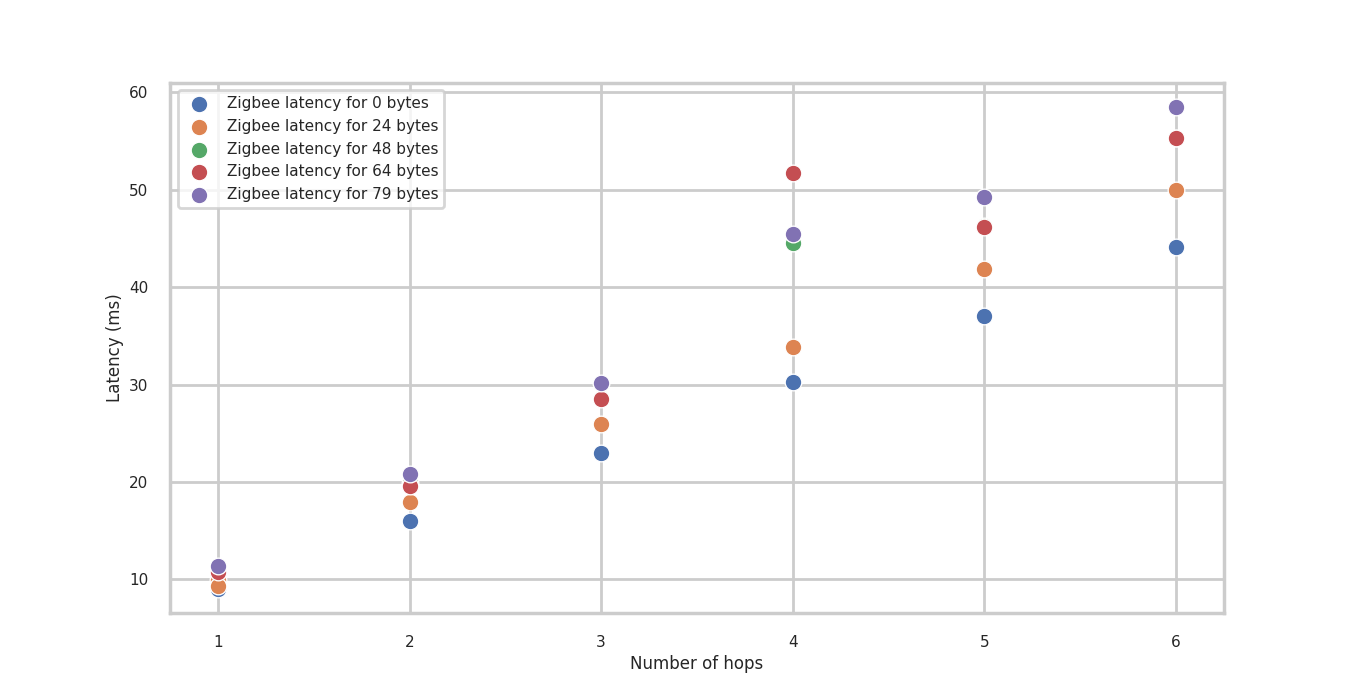
\includegraphics[scale=0.45]{images/Zigbee_Latency_all.png}
    \caption{Latency in Zigbee network dependent on the number of hops.}
    \label{fig:zigbee_latency_all}
\end{figure}

The single hop delay in Zigbee differs from the one estimated for 
Thread. In this case the latency varies between \textbf{9 and 11.5 milliseconds}, which is higher than for Thread. The relation between
latency and the payload length is shown in 
Figure \ref{fig:zigbee_latency_length}.

\begin{figure}[H]
    \centering
    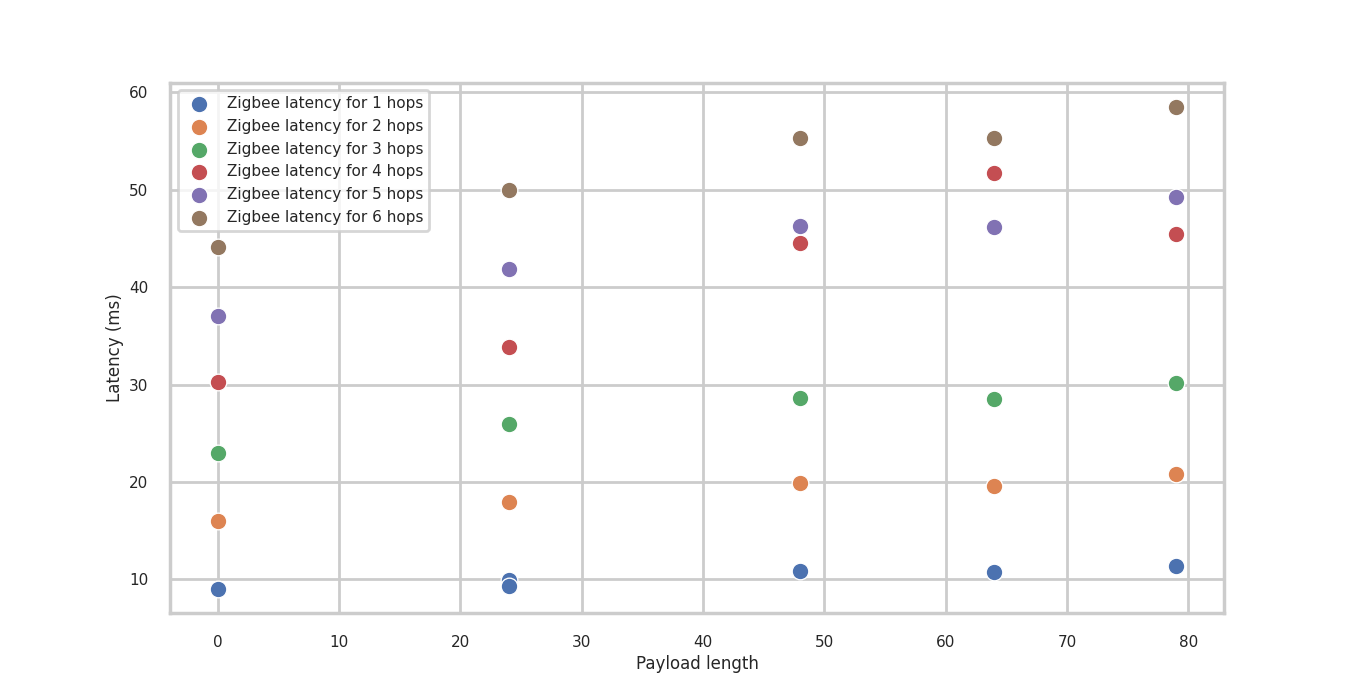
\includegraphics[scale=0.45]{images/Zigbee_Latency_vs_length.png}
    \caption{Latency in Zigbee network dependent on the payload length. }
    \label{fig:zigbee_latency_length}
\end{figure}

\newpage
\section{Throughput}
\label{sec:throughput}

Throughout the experiments, throughput was computed as a ratio of sent
bites and the full time of test execution. This is expressed as

\begin{equation}
Throughput = \frac{payload\textunderscore length \cdot 8}{execution\textunderscore time} [kbps].
\label{eq:throughput}
\end{equation}

Before diving into the results, some conclusions can be noticed by
looking at the equation \ref{eq:throughput}. Throughput depends on
two factors: length of the payload and time of test execution.
When payload length increases, throughput increases as well. If 
execution time is higher, throughput decreases.

The execution time of test consists of the latency multiplied by
a number of sent packets and time spent on data processing. The latter
includes delays introduced by: buffers copying, packet scheduling and 
the overall network stack processing.

\subsection{Throughput in Thread networks}

Following plots (\ref{fig:thread_throughput_all}, 
\ref{fig:thread_throughput_length}) show the throughput in Thread 
network relatively to the number of hops or payload length. As
determined at the beginning of this section, throughput is
directly proportional to the payload length and inversely proportional
to the latency (which depends directly on the number of hops).

\begin{figure}[H]
    \centering
    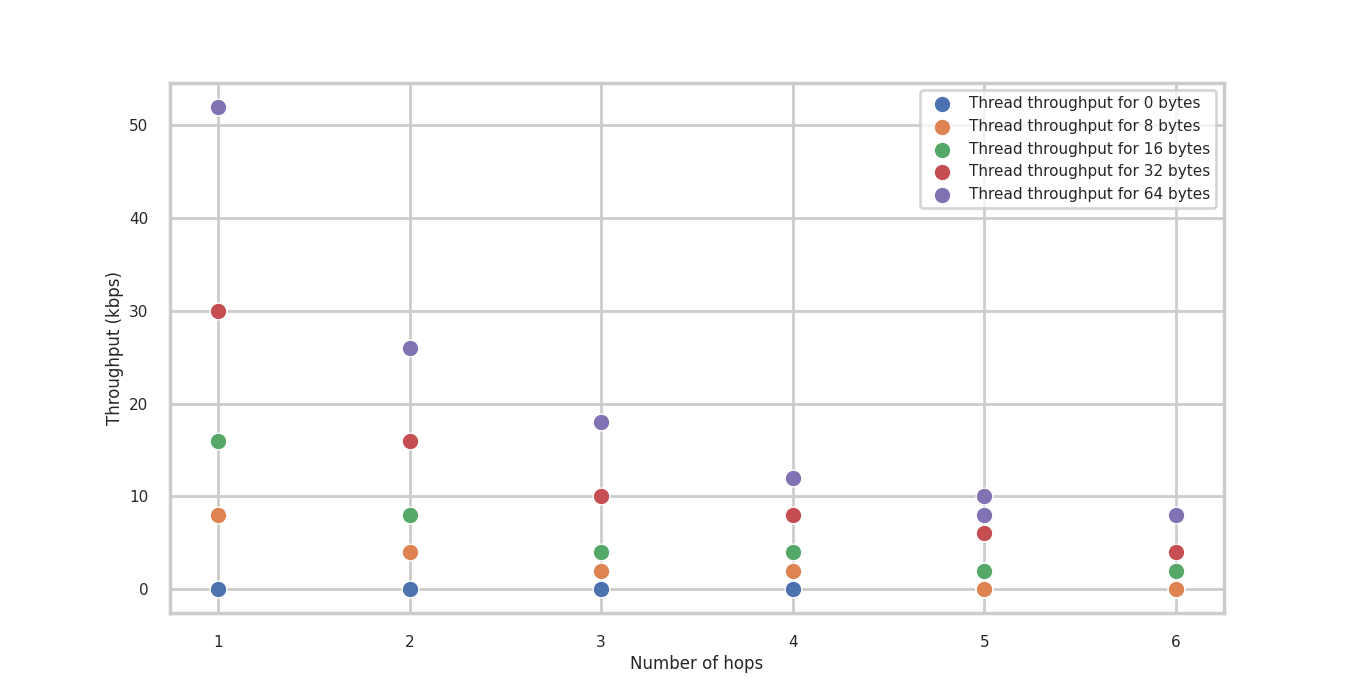
\includegraphics[scale=0.45]{images/Thread_Throughput_all.png}
    \caption{Throughput in Thread network dependent on the number of hops.}
    \label{fig:thread_throughput_all}
\end{figure}

\begin{figure}[H]
    \centering
    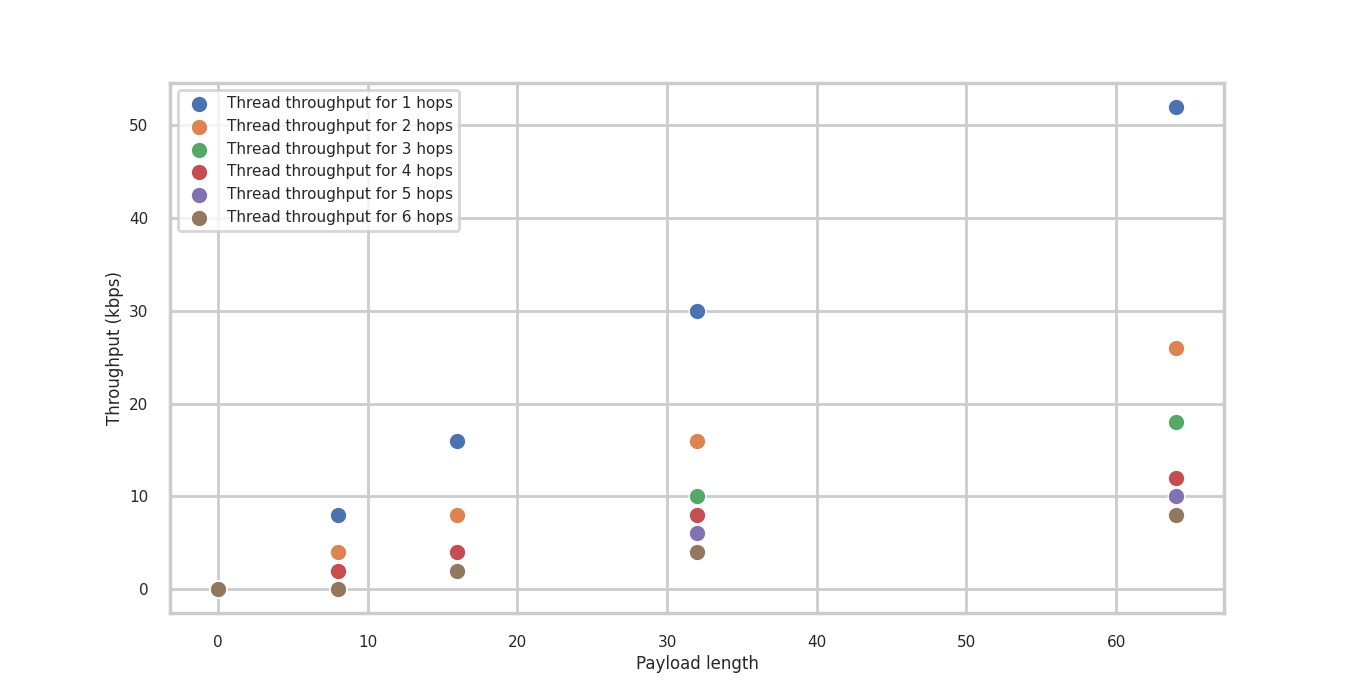
\includegraphics[scale=0.45]{images/Thread_Throughput_vs_length.png}
    \caption{Throughput in Thread network dependent on the payload length. }
    \label{fig:thread_throughput_length}
\end{figure}

The minimum throughput in Thread network for non-zero bytes long payload and 1 hop is \textbf{4}kbps. The maximum of \textbf{52kbps} was obtained
for 1 hop and 64 bytes long payload. It is worth to mention that every case which uses
0 bytes long payload yields 0 kbps payload.


\subsection{Throughput in Zigbee networks}

The results of throughput measurements of Zigbee network are depicted
in figures \ref{fig:zigbee_throughput_all} and \ref{fig:zigbee_throughput_length}. The dependencies of
throughput and packet length or execution time are the same as
for Thread. The minimum value of throughput (0kbps) as well as for
Thread is received when 0 bytes long payload is sent. The minimum value for non-zero bytes long payload (received for 8 bytes and 1 hop) is \textbf{3} kbps. The maximum
throughput in Zigbee network, received for 1 hop and 64 bytes long payload equals \textbf{44kbps}.


\begin{figure}[H]
    \centering
    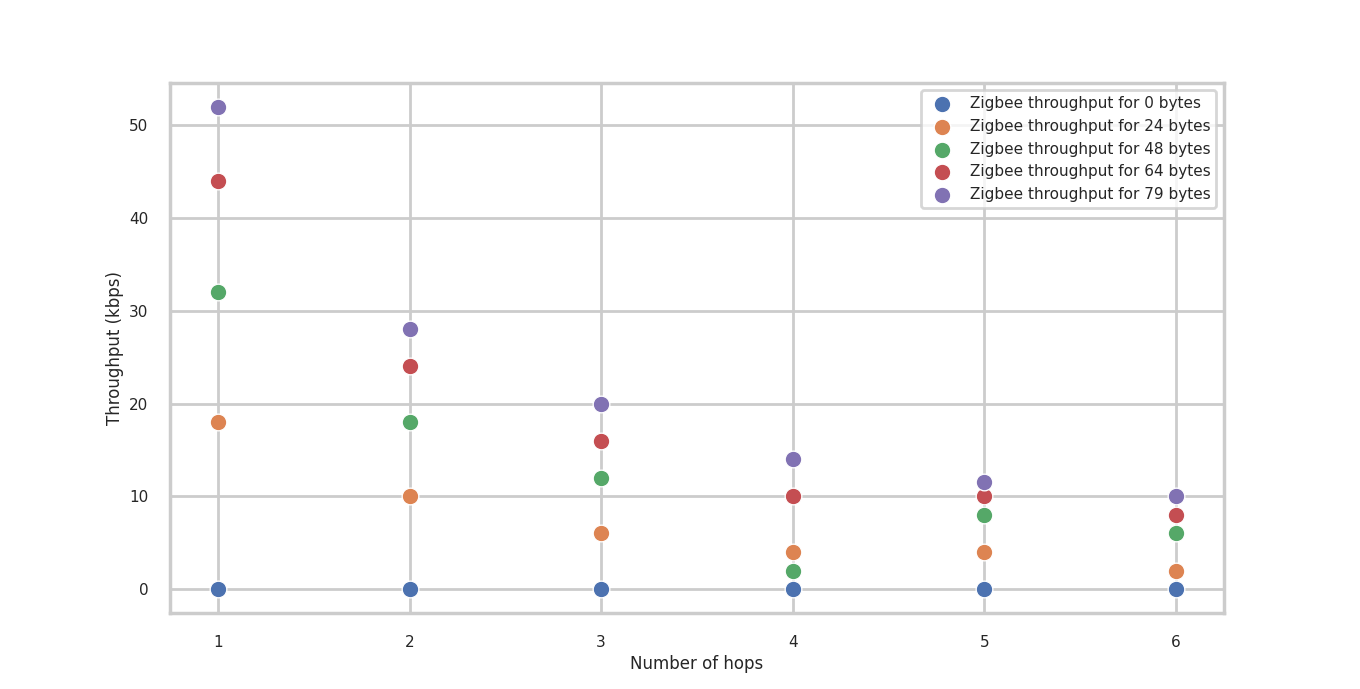
\includegraphics[scale=0.45]{images/Zigbee_Throughput_all.png}
    \caption{Throughput in Zigbee network dependent on the number of hops.}
    \label{fig:zigbee_throughput_all}
\end{figure}

\begin{figure}[H]
    \centering
    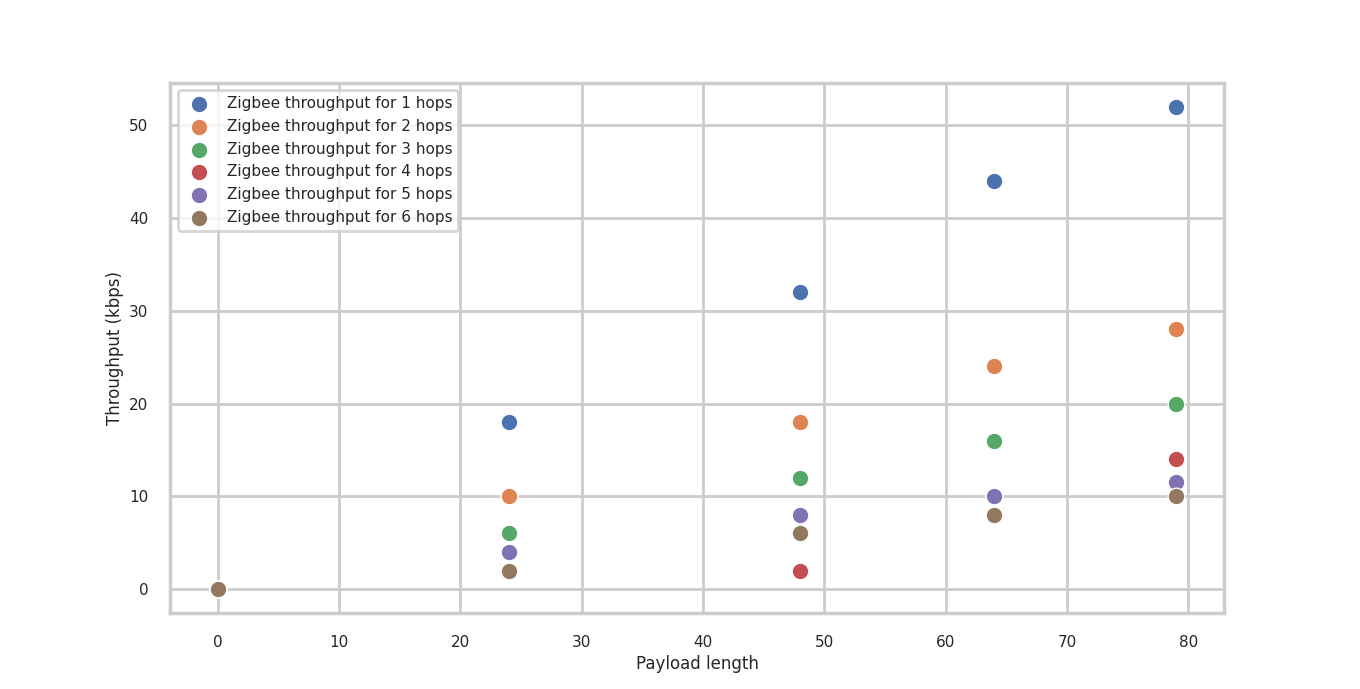
\includegraphics[scale=0.45]{images/Zigbee_Throughput_vs_length.png}
    \caption{Throughput in Zigbee network dependent on the payload length. }
    \label{fig:zigbee_throughput_length}
\end{figure}

\section{Performance comparison}
\label{sec:performance_comparison}

As shown in sections \ref{sec:latency} and \ref{sec:throughput}, the 
two fundamental metrics of network protocol performance obey the
similar principles. It is not surprising, because both tested 
technologies are built upon the same MAC layer. This implies that none
of them cannot go beyond IEEE 802.15.4 constraints.

For latency, as well as for throughput measurements, Thread network 
performs better. Figure \ref{fig:thread_vs_zigbee_latency} presents
latency of 24 bytes long payload for these two protocols and the 
throughput is shown in \ref{fig:thread_vs_zigbee_throughput}. The tests
showed that Thread is significantly faster than Zigbee.


\begin{figure}[H]
    \centering
    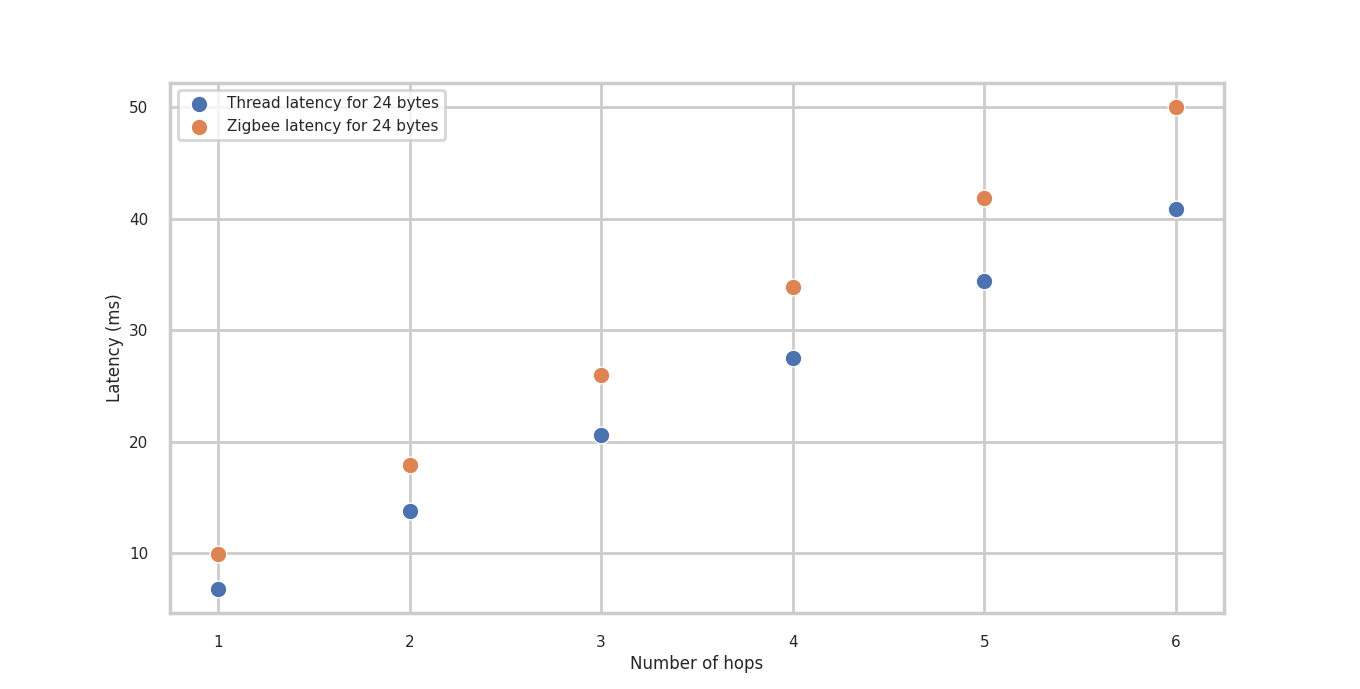
\includegraphics[scale=0.45]{images/Thread_vs_Zigbee_Latency.png}
    \caption{Latency comparison betwen Thread and Zigbee.}
    \label{fig:thread_vs_zigbee_latency}
\end{figure}

The comparison
between most representative results alongside with calculated differences are shown in the table 
\ref{table:comparison}.

\begin{figure}[H]
    \centering
    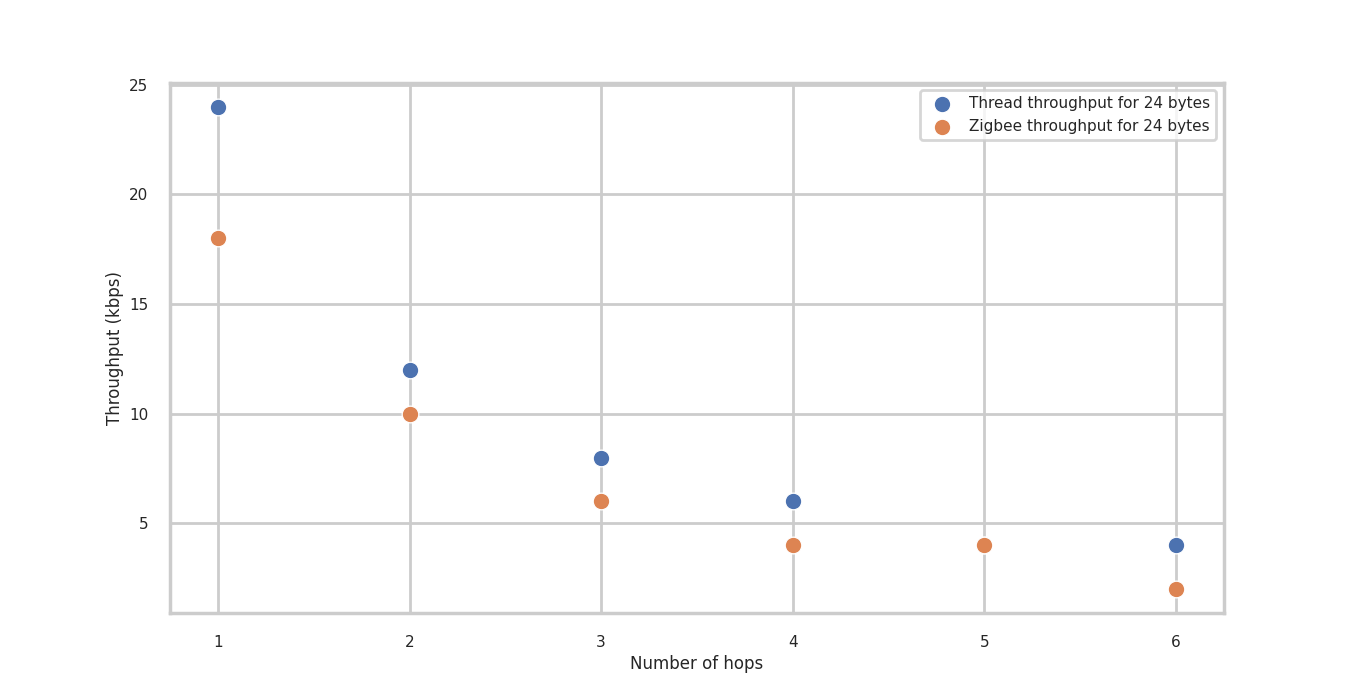
\includegraphics[scale=0.45]{images/Thread_vs_Zigbee_Throoughput.png}
    \caption{Throughput comparison between Thread and Zigbee.}
    \label{fig:thread_vs_zigbee_throughput}
\end{figure}



\begin{table}[H]
\centering
\begin{tabular}{|c|c|c|c|}
\hline
Metric    & Thread & Zigbee & Difference        \\
\hline
\multicolumn{4}{c}{0 bytes, 1 hop}     \\
\hline
Latency (ms)   &   5.74     &   9.00     &  3.26 (56.8\%)               \\
Throughput (kbps) &   0     &    0    &          (0\%)         \\
\hline
\multicolumn{4}{c}{24 bytes, 1 hop}    \\
\hline
Latency (ms)   &  6.76      &   9.95     &     3.19 (47.2\%)             \\
Throughput (kbps) &   24     &    18    &     6  (33.3\%)            \\
\hline
\multicolumn{4}{c}{64 bytes, 1 hop}    \\
\hline
Latency (ms)   &   8.33     &   10.76     &    2.43  (29.2\%)          \\
Throughput (kbps) &   52     &    44    &   8   (18.2\%)            \\
\hline
\end{tabular}
\caption{Comparison of latency and throughput for chosen number of hops and payload length between Thread and Zigbee.}
\label{table:comparison}
\end{table}

The performance differences between Zigbee and Thread are significantly
higher for shorter payload lengths. Taking into account that tests
were executed on the same hardware and both protocols use IEEE 802.15.4
MAC layer, it can be assumed that for a packet of given length, the 
time in the air is the same. That said, the factor affecting the
packets delay in Zigbee network is probably associated with data 
processing. Working on a packet in Zigbee takes longer than in
Thread.
